\documentclass[11pt]{article} % For LaTeX2e
\usepackage{nips12submit_e,times}
%\documentstyle[nips12submit_09,times,art10]{article} % For LaTeX 2.09

%\usepackage[usenames,dvipsnames]{color}

\usepackage[utf8]{inputenc}
\usepackage[T1]{fontenc}
\usepackage{textcomp}
\usepackage[scaled=0.8]{beramono}

\usepackage{caption}
\usepackage{subcaption}
\usepackage{wrapfig}
\usepackage{amsmath,amssymb}
\usepackage{array}
\usepackage{tabularx}
\usepackage{booktabs}
\usepackage{graphicx}

\usepackage{url}
\usepackage[hyperfootnotes=false,citecolor=RedOrange,linkcolor=RoyalBlue,urlcolor=DarkOrchid,colorlinks]{hyperref}
\usepackage[all]{hypcap}

\newcommand{\todo}[1]{\noindent\texttt{\color[rgb]{0.5,0.1,0.1} TODO: #1}}

\newcommand{\sectref}[1]{\mbox{Section~\ref{#1}}}
\newcommand{\figref}[1]{\mbox{Figure~\ref{#1}}}
\newcommand{\tabref}[1]{\mbox{Table~\ref{#1}}}
\renewcommand{\sectref}[1]{\hyperref[#1]{\mbox{Section~\ref*{#1}}}}
\renewcommand{\figref}[1]{\hyperref[#1]{\mbox{Figure~\ref*{#1}}}}
\renewcommand{\tabref}[1]{\hyperref[#1]{\mbox{Table~\ref*{#1}}}}

\title{Simulating disease spread in social networks\thanks{Final project
for the course ``Introduction to Social Network Analysis'' (Spring
Semester 2012).}}

\author{
Alkis Gkotovos\\
Department of Computer Science, ETH Zurich\\
\texttt{alkisg@student.ethz.ch}
}

\nipsfinalcopy % Uncomment for camera-ready version

\begin{document}

\maketitle

\begin{abstract}
In this report I present a model, similar to the common SIR and SIS models,
which can be used to simulate the spread of an infectious disease in
social networks. I also present and discuss simulation results on three
types of generated networks for different choices of graph parameters.
\end{abstract}

\section{Introduction}
The spread of diseases in human networks is an interesting research topic, both
for historical reasons (e.g. analysis of the ``Black Death'' pandemic in the
14th century~\cite{blackdeath}), as well as for dealing with contemporary or
future epidemics (e.g. AIDS spread in Africa~\cite{aids}). Furthermore, the
concept of network diffusion can be generalized to other types of phenomena,
like the spread of computer viruses in e-mail networks~\cite{email}, or even
the spread of behavioral phenomena, also referred to as
\emph{social contagion}~\cite{contagion}.

To fully analyze disease spread in networks, one needs to know in detail the
characteristics of the disease itself (transimission, active period, etc.),
as well as have available a fine-grained network of interactions. Moreover, the network
information required may depend on the disease attributes (e.g. for an airborne virus
it may be important to include interactions in public transports). Since this
kind of information is usually not available, there have been proposed a
number of simple models that can be used as a first step for simulating disease
spread. Two of them, commonly found in the literature, are the SIR and SIS
models~\cite{easley, newman}.

Both models assume discrete time steps and represent each node of the network
as a state machine that can be in exactly one state at each time step. In the
SIR model healthy nodes that can be infected are in the \emph{susceptible} ($S$)
state, infected nodes are in the \emph{infected} (I) state, and nodes that have
gone through the infection and cannot be infected again are in the \emph{removed}
($R$) state. At every time step, an $I$ node may independently infect each of
its $S$ neighbors with probability $p_I$. Each $I$ node stays infected for
$t_I$ steps and, afterwards, transitions into the $R$ state.
The SIS model is very similar and only differs in the fact that nodes return
to the $S$ state after the infection is over, instead of transitioning to the
$R$ state.

\section{Model description}
I introduce a new disease spread model, called SIMR, which is very similar to
the SIR/SIS models, albeit slightly more complex. The rationale behind extending
these models is twofold. First, the SIR/SIS models only allow transitions out
of the $I$ state after the whole infectious period has passed, which I find to be
constraining, because it defines a completely fixed period during which a node is
infected. Second, in choosing one of the two models, one has to stick with
always transitioning to either the $S$ state or the $R$ state after the infection
is over, which I also find inflexible.

With the above ideas in mind, the SIMR model works as follows:
\begin{itemize}
\item As in the SIR/SIS models, healthy nodes are in the $S$ state and infected
nodes are in the $I$ state. Also, as before, an $I$ node may infect any of its
$S$ neighbors with probability $p_I$.
\item The first extension is that, although an $I$ node stays infected for $t_I$
time steps, it can transition to the $R$ state with probability $p_R$ at each
time step of the infection. This, in a sense, models the fact that an infected
person may pass away at any point during the infected period with a certain
probability.
\item The second extension is that the transition after the infection is over
is not fixed, but is determined probabilistically. In particular, the previously
infected node transitions to an \emph{immune} ($M$) state with probability $p_M$,
or otherwise returns to the $S$ state. The $M$ state is similar to the $R$
state from an operational perspective, but is semantically different.
\end{itemize}

\section{Implementation and experimental setup}
The model presented in the previous section can be easily implemented in any
programming language with graph support. I chose to use Python, because it is
easy to program and test with, has good graph support and nice visualization
libraries.
To simulate the model, I chose to use three popular classes of randomly generated
networks whose characteristics are briefly reviewed below. Subsequently, I
describe the way that simulations are carried out.

\subsection{Implementation}
I implemented the SIMR model in Python using
NetworkX\footnote{\url{http://networkx.lanl.gov/}} for graph
generation and manipulation, as well as
matplotlib\footnote{\url{http://matplotlib.sourceforge.net/}} for plotting.
In short, my class \texttt{Simr} encapsulates the
disease spread model by storing the four model parameters $p_I$, $t_I$, $p_R$
and $p_M$, keeping track of the state of each node, and updating the node state
at each time step accordingly. In addition, I have
written code for visualizing the network state and automatically running
and plotting multiple simulations. The Python module \texttt{diffuse.py}
containing all code I have written for this project can be found on
GitHub\footnote{\url{https://github.com/3lectrologos/sna}}.

\subsection{Random graph models}
\noindent\textbf{Erdős–Rényi model.} The Erdős–Rényi (ER) model~\cite{erdos} is
probably the simplest possible model for generating a random graph. The
construction process of the graph consists in specifying the number of
nodes $n$ and, subsequently, independently adding every possible edge
with probability $p$. We expect that the notion of \emph{percolation
threshold}, i.e. the value of $p$ that, for given $n$, differentiates
between a single large graph component and a number of small graph
components, plays an important role in disease spread. I will refer to a
generated graph of this class as ER$(n, p)$.

\noindent\textbf{Watts-Strogatz model.} The Watts-Strogatz (WS)
model~\cite{watts} was proposed as a more realistic model for generating graphs
that have \emph{small-world} properties, i.e. large clustering combined with
short average path lengths. The graph is constructed by starting with a ring
topology of $n$ nodes, where each node is connected to its $k$ closest neighbors
in the ring. Subsequently, every existing edge is rewired withe probability $p$.
We expect that disease spread will be more severe in such a network, because
of the small-world properties. I will refer to a generated graph of this class
as WS$(n, k, p)$.

\noindent\textbf{Barabási-Albert model.} The Barabási-Albert (BA)
model~\cite{barabasi} aims to generate graphs with \emph{scale-free} degree
distributions, which may be more realistic than the degree distributions of
WS graphs. A graph is generated by implementing the notion of
\emph{preferential attachment}. In particular, for generating a graph with
$n$ nodes, one node is added at a time and it is connected to $m$ of the
existing nodes with probability proportional to the degree of each existing
node. It follows that the model favors the creation of hubs, i.e. nodes that
accumulate a lot of edges, which is expected to play a role in disease spread
(for example, removing a few large hubs from the network might make a big
difference). I will refer to a generated graph of this class
as BA$(n, m)$.

\subsection{Types of experiments}
To obtain the results in the following section, two types of simulations are
used. The first consists in simulating the network only once, starting with
a specified percentage of infected nodes and terminating as soon as
there are no more infected nodes, which means that the system has reached a
fixed point. For this type of simulation, I plot the percentage of healthy,
infected, immune, and dead nodes as a function of time steps and call it an
\emph{evolution plot}, because it depicts the evolution of a single disease
spread scenario against time.

The second type of simulation consists in carrying out a number of iterations
of the above procedure for a range of different values of a specific network
parameter. In this case, I plot the average of the healthy, infected,
and immune node percentages at the end of each iteration, as well as the average
of the maximum infected node percentage during each iteration, as a function of
the specified network parameter. I call this kind of plot a
\emph{summary plot}, because it does not contain detailed information about
the spread evolution at each iteration.

For all simulations I fix the SIMR model parameters to the values shown
in \tabref{tab:params}. This is done to mainly focus on comparing how the
graph properties affect the disease spread. Furthermore, all simulations start
with 5\% randomly chosen infected nodes.

\begin{table}[t]
  \centering
  \caption{SIMR model parameters used in the simulations.}
  \label{tab:params}
  \begin{tabularx}{\textwidth}{*{4}{>{\centering\arraybackslash}X}}
    \toprule
    Probability of infection ($p_I$) & Length of infection in time steps ($t_I$) &
    Probability of removal ($t_R$) & Probability of immunity ($p_M$)\\
    \midrule
    0.05 & 6 & 0.05 & 0.2\\
    \bottomrule
  \end{tabularx}
\end{table}

\section{Results}
Before starting the simulations on large graphs, it is interesting to visualize
the spread evolution on a smaller graph. \figref{fig:er_graph_evo} shows
four evolution stages of a simulation on a fairly dense ER(50, 0.3) graph.
In panel (a) most nodes are healthy (blue) and 5\% of them, i.e. 3 nodes, are
infected (green). After 10 steps, in panel (b) the disease has already spread
to most of the network and there are already a few removed (gray) and immune (gold)
nodes. In panel (c) we see that after 20 steps the disease has declined significantly,
leaving behind a number of removed nodes. Finally, in panel (d) the simulation has
ended after 35 steps, since there are no more infected nodes left.

As mentioned before, the spread evolution for larger graphs can be visualized
more conveniently using evolution plots. \figref{fig:er_evo} shows two such
plots for two ER graphs, one significantly denser than the other. Two important
graph metrics for these and other graphs used in following simulations are
recorded in \tabref{tab:metrics}. Note that both evolution plots exhibit
a clear disease outbreak period, as well as a slow decline after that.
As expected, the outbreak in the denser graph of the two is both faster and
significantly more severe (in terms of infection peak and number of removed nodes
at the end) than the one in the sparser graph.

\begin{figure}[tbp]
  \begin{subfigure}[b]{0.5\textwidth}
    \centering
    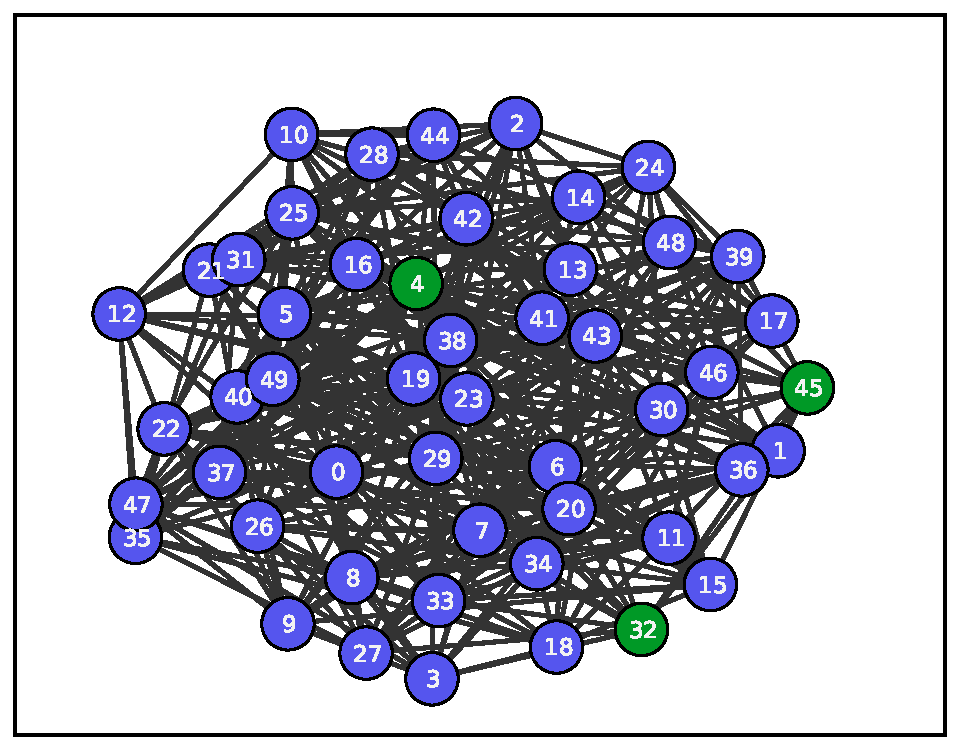
\includegraphics[width=\textwidth]{figures/evo_ER_50_03_init}
    \caption{Initial graph state}
  \end{subfigure}
  \begin{subfigure}[b]{0.5\textwidth}
    \centering
    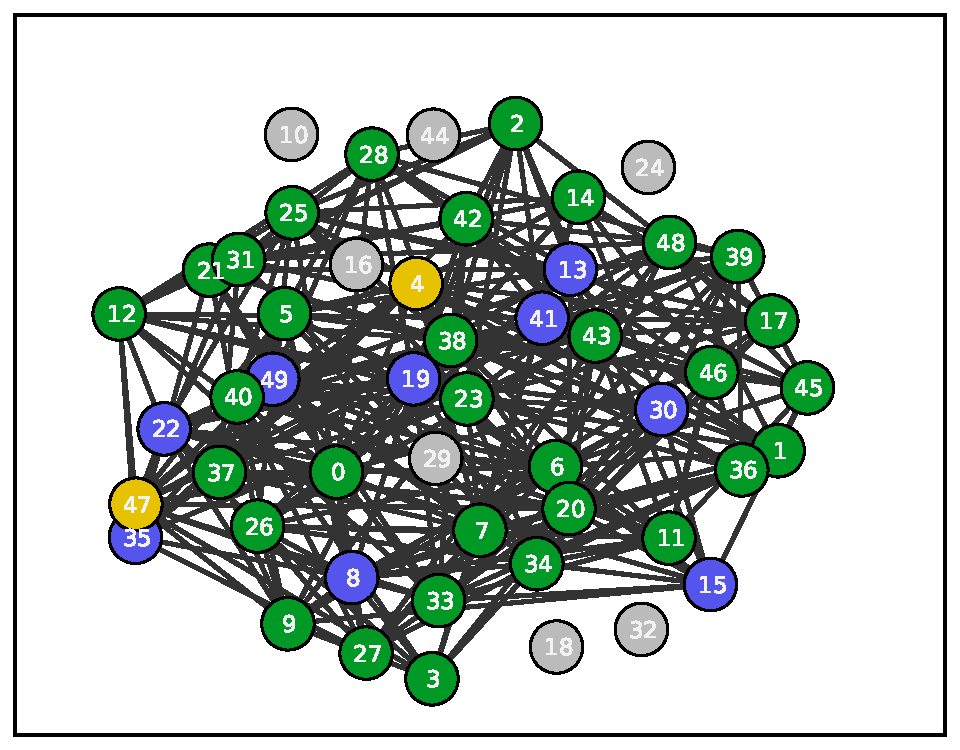
\includegraphics[width=\textwidth]{figures/evo_ER_50_03_10}
    \caption{Graph state after 10 steps}
  \end{subfigure}
  \begin{subfigure}[b]{0.5\textwidth}
    \centering
    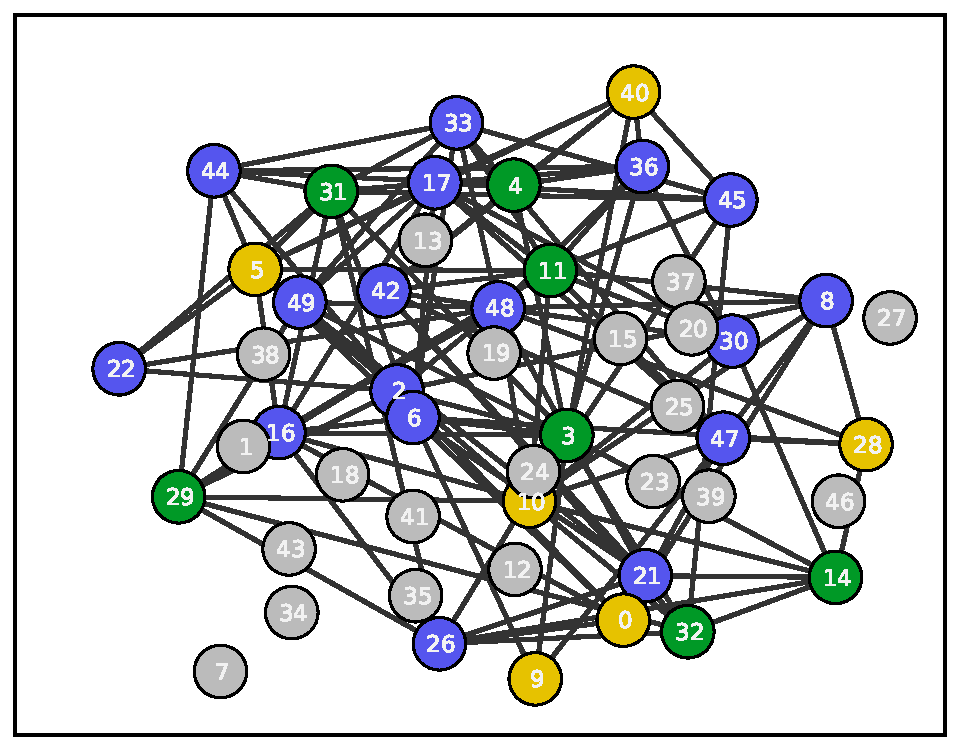
\includegraphics[width=\textwidth]{figures/evo_ER_50_03_20}
    \caption{Graph state after 20 steps}
  \end{subfigure}
  \begin{subfigure}[b]{0.5\textwidth}
    \centering
    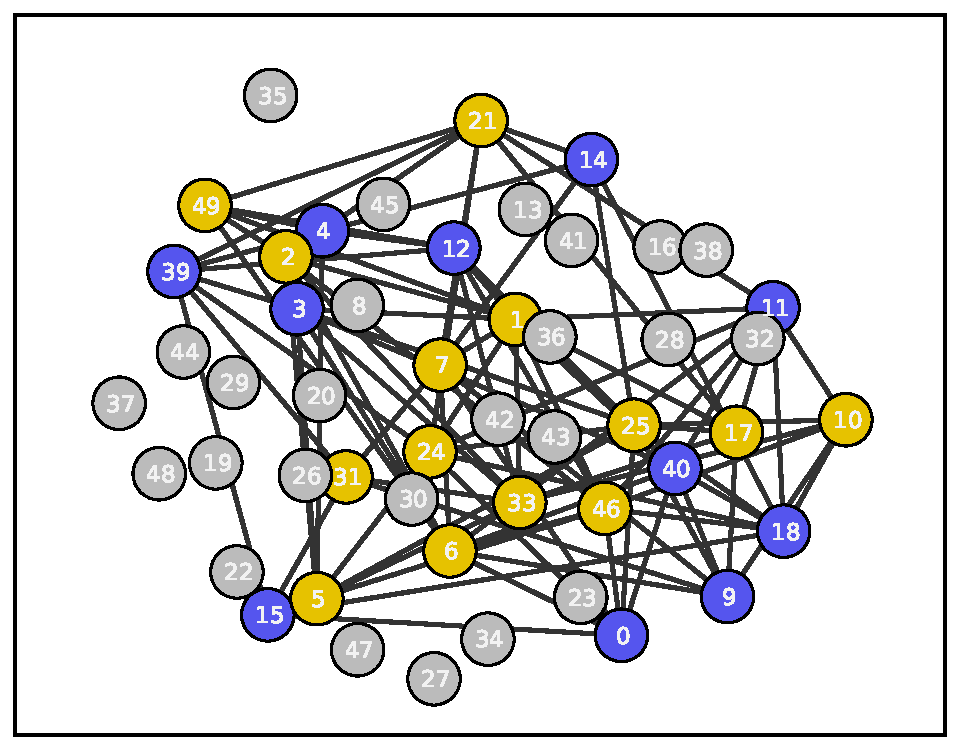
\includegraphics[width=\textwidth]{figures/evo_ER_50_03_final}
    \caption{Final graph state after 35 steps}
  \end{subfigure}
  \caption{Different stages of the simulation for an ER(50, 0.3) graph.}
  \label{fig:er_graph_evo}
\end{figure}

\begin{figure}[tbp]
  \begin{subfigure}[b]{0.5\textwidth}
    \centering
    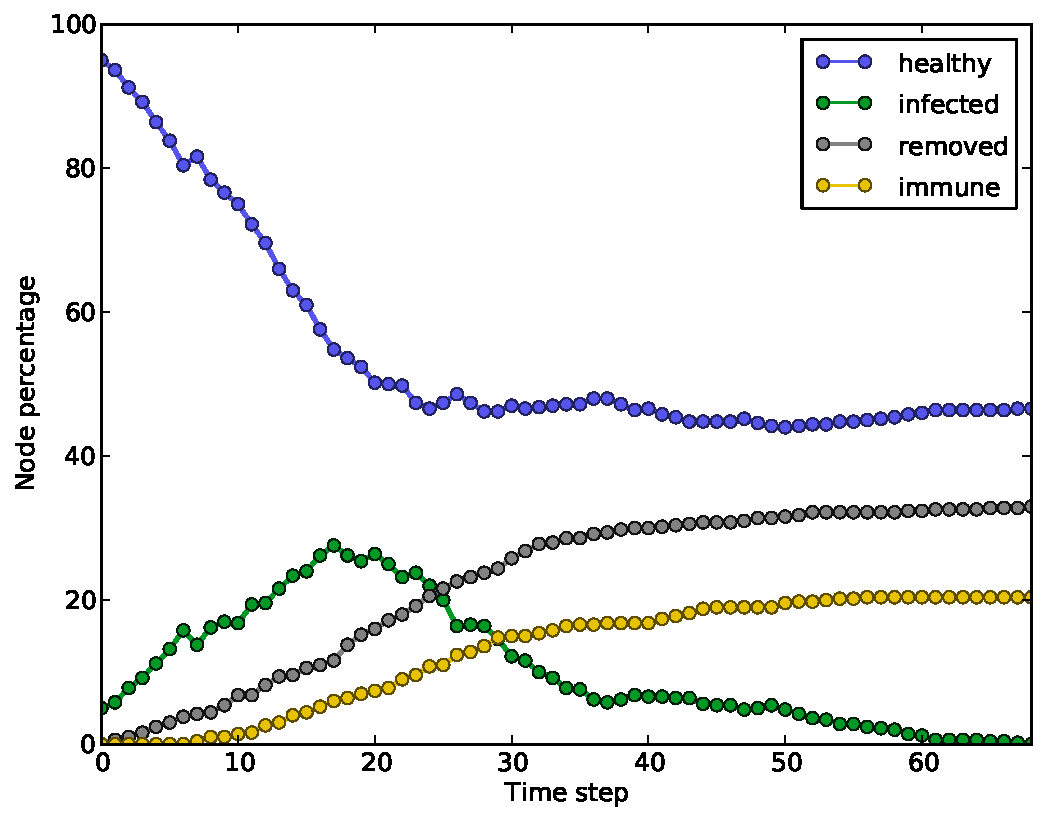
\includegraphics[width=\textwidth]{figures/evo_ER_500_0015}
  \end{subfigure}
  \begin{subfigure}[b]{0.5\textwidth}
    \centering
    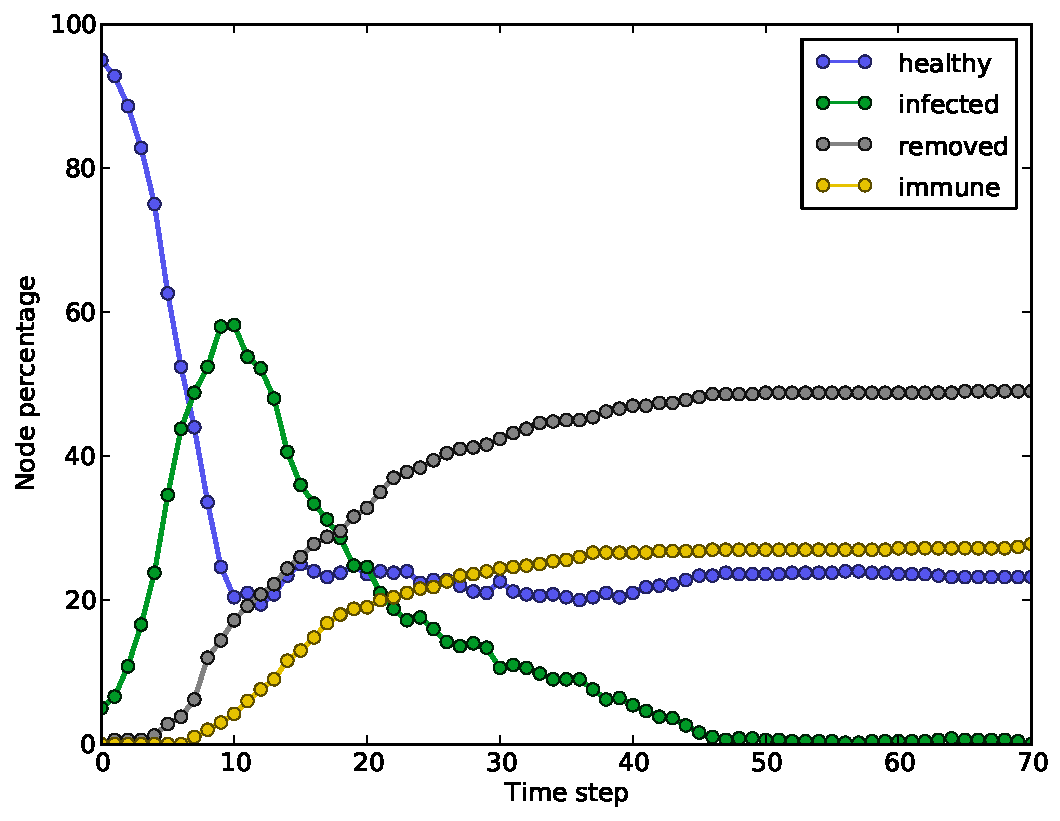
\includegraphics[width=\textwidth]{figures/evo_ER_500_003}
  \end{subfigure}
  \caption{Evolution plots for an ER(500, 0.015) graph (left) and an
    ER(500, 0.03) graph (right).}
  \label{fig:er_evo}
\end{figure}

\begin{table}[tb]
  \centering
  \caption{Graph measures of the graphs used in the simulations.}
  \label{tab:metrics}
  \begin{tabularx}{\textwidth}{l  *{6}{>{\centering\arraybackslash}X}}
    \toprule
    \textbf{Graph} & \textbf{Avg. clustering coeff.} & \textbf{Avg. shortest path length}\\
    \midrule
    ER(500, 0.015) & 0.016 & 3.29\\
    \midrule
    ER(500, 0.030) & 0.032 & 2.60\\
    \midrule
    WS(500, 15, 0.1) & 0.510 & 3.30\\
    \midrule
    WS(500, 30, 0.1) & 0.540 & 2.55\\
    \midrule
    BA(500, 3) & 0.046 & 3.23\\
    \midrule
    BA(500, 7) & 0.081 & 2.56\\
    \bottomrule
  \end{tabularx}
\end{table}

\begin{wrapfigure}[16]{R}{0.5\textwidth}
  \centering
  \vspace{-7pt}
  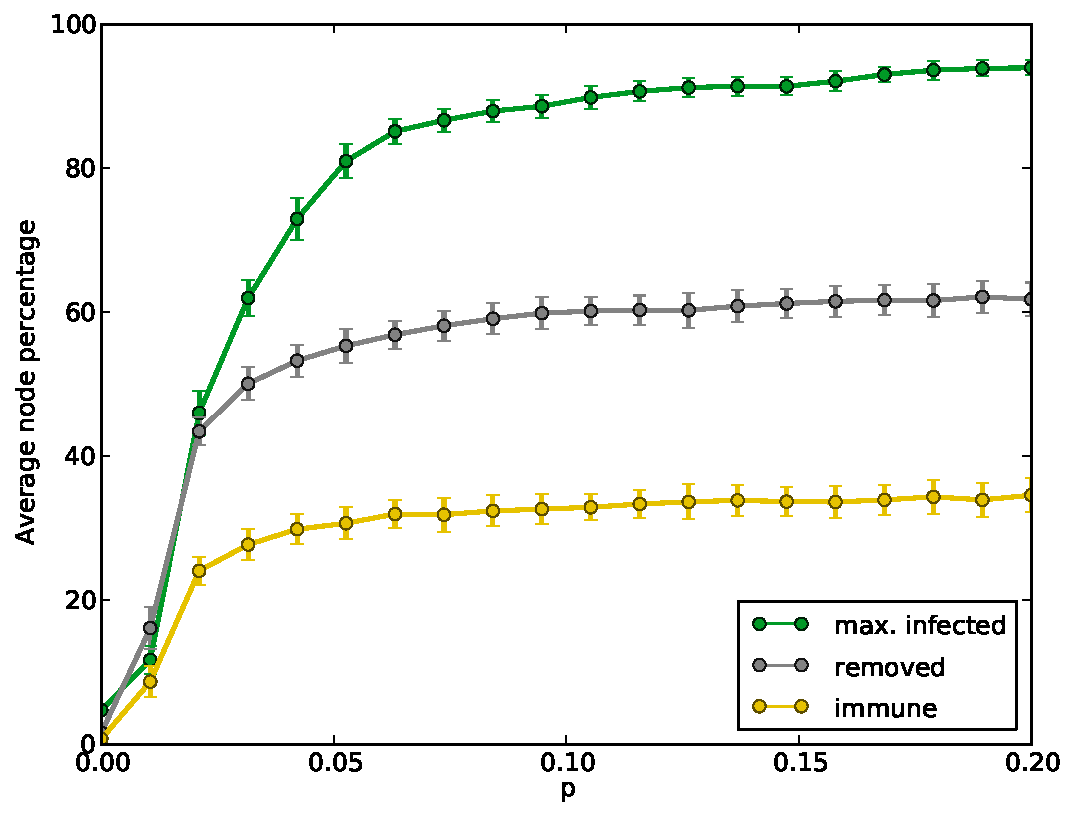
\includegraphics[width=0.5\textwidth]{figures/sum_ER_500_p}
  \vspace{-17pt}
  \caption{Summary plot for ER(500, p).}
  \label{fig:er_sum}
\end{wrapfigure}

The effect of graph density on the severity of disease spread is seen more
clearly when using a summary plot, like the one shown in
\figref{fig:er_sum}. More specifically, this plot depicts average node
percentages for different values of the ER graph parameter $p$, using
100 simulations per tested value. (The same number of simulations is carried
out for all summary plots that will follow.) It is obvious that for larger values
of $p$, i.e. denser graphs, the disease spread becomes more pronounced.
More importantly, note that, since $n = 500$, the percolation threshold of
these graphs is about 0.02, which is notably the value around which the
disease spread starts to increase significantly. Also, it is evident that
at $p = 0.1$ the disease has almost reached its maximum spread and further
increasing $p$ does not seem to make a big difference with respect to the
measured quantities.

Next, I have chosen two sets of WS graph parameters, such that the average
shortest path lengths of the resulting graphs
are about the same as the previously examined ER graphs, in order to
examine the clustering (small-world) effect. \tabref{tab:metrics} shows that
the average shortest path lengths are very close to the ones of the ER graphs,
but the clustering coefficients are vastly larger. The corresponding
evolution plots are shown in \figref{fig:ws_evo}. Note that the disease
outbreak is clearly larger in the WS graphs compared to the plots of
\figref{fig:er_evo}, which validates the hypothesis that a large clustering
coefficient boosts disease spread.

\begin{figure}[b]
  \begin{subfigure}[b]{0.5\textwidth}
    \centering
    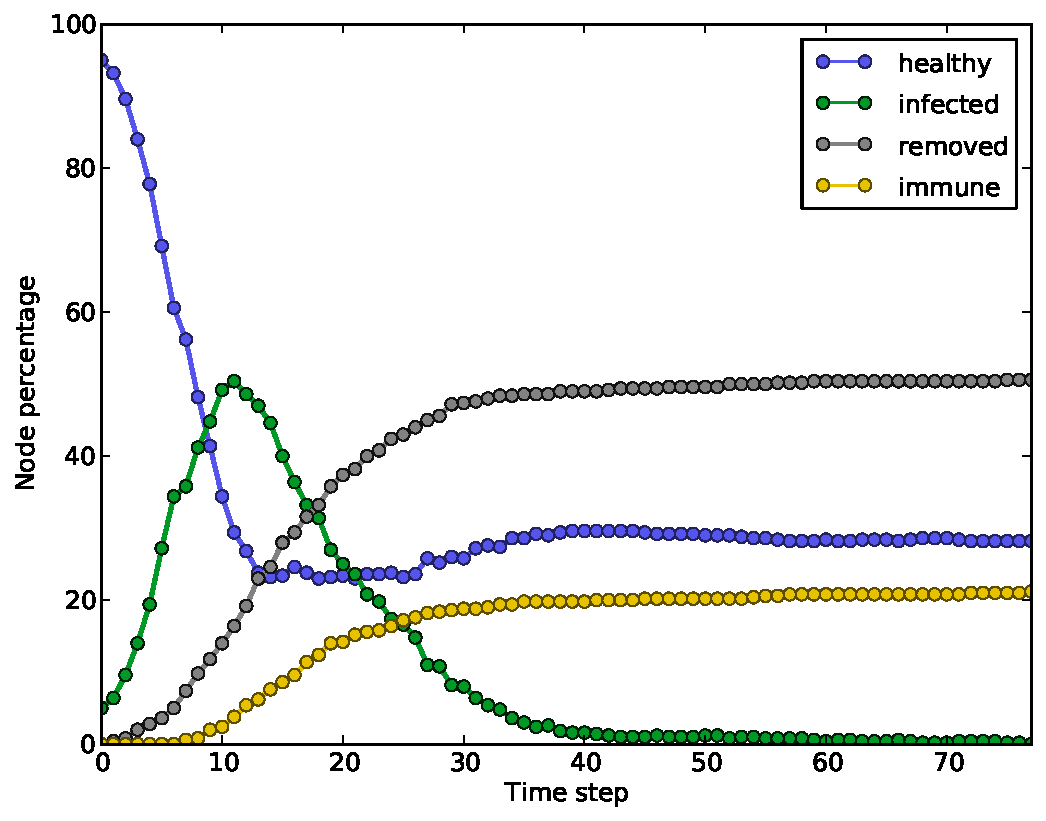
\includegraphics[width=\textwidth]{figures/evo_WS_500_15_01}
  \end{subfigure}
  \begin{subfigure}[b]{0.5\textwidth}
    \centering
    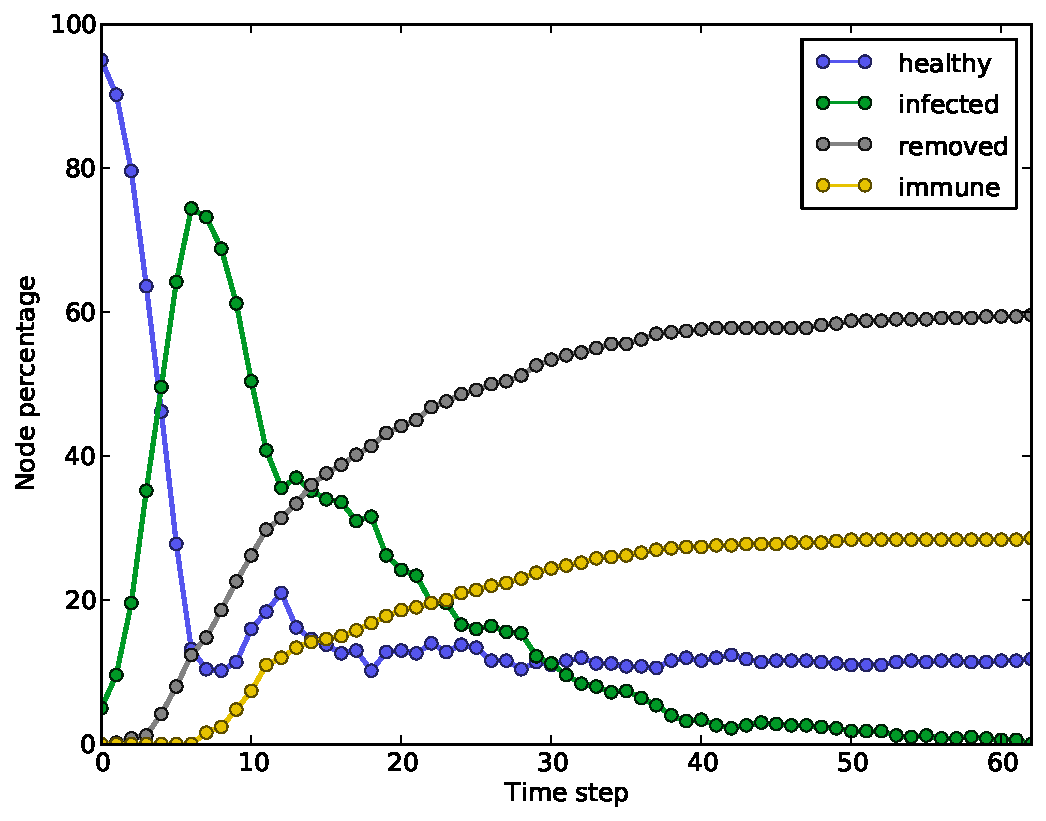
\includegraphics[width=\textwidth]{figures/evo_WS_500_30_01}
  \end{subfigure}
  \caption{Evolution plots for a WS(500, 20, 0.1) graph (left) and a
    WS(500, 40, 0.1) graph (right).}
  \label{fig:ws_evo}
\end{figure}

\begin{figure}[tb]
  \begin{subfigure}[b]{0.5\textwidth}
    \centering
    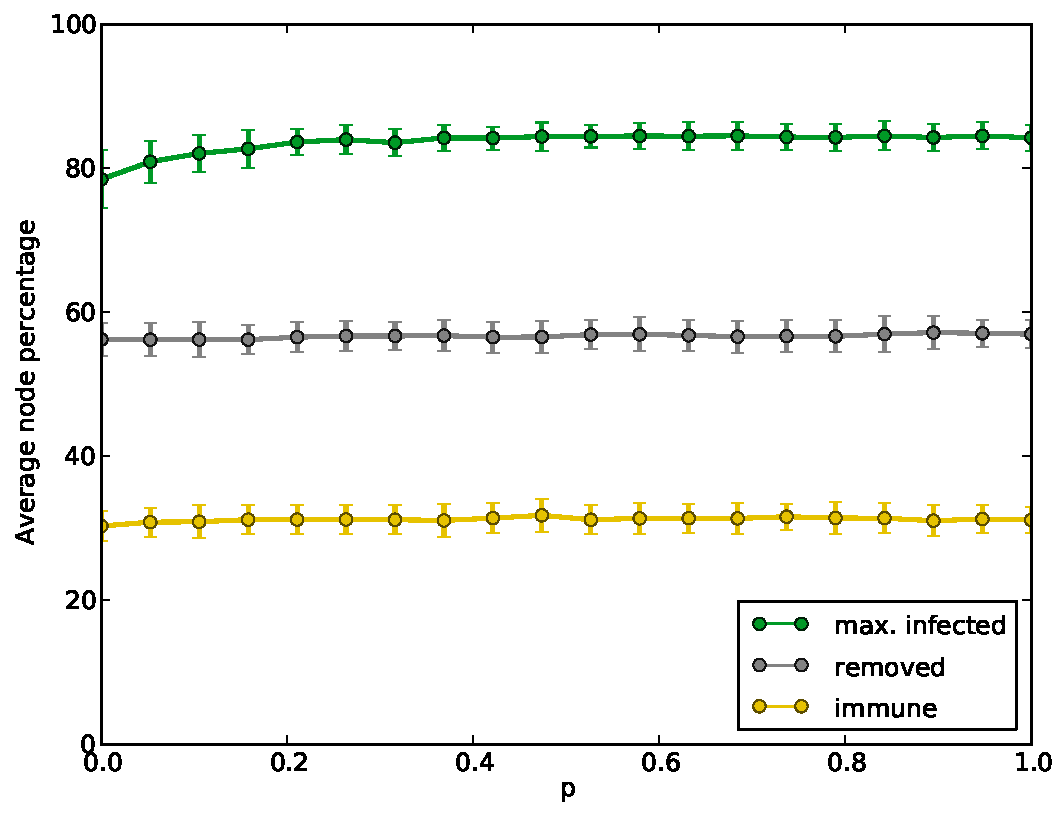
\includegraphics[width=\textwidth]{figures/sum_WS_500_25_p}
  \end{subfigure}
  \begin{subfigure}[b]{0.5\textwidth}
    \centering
    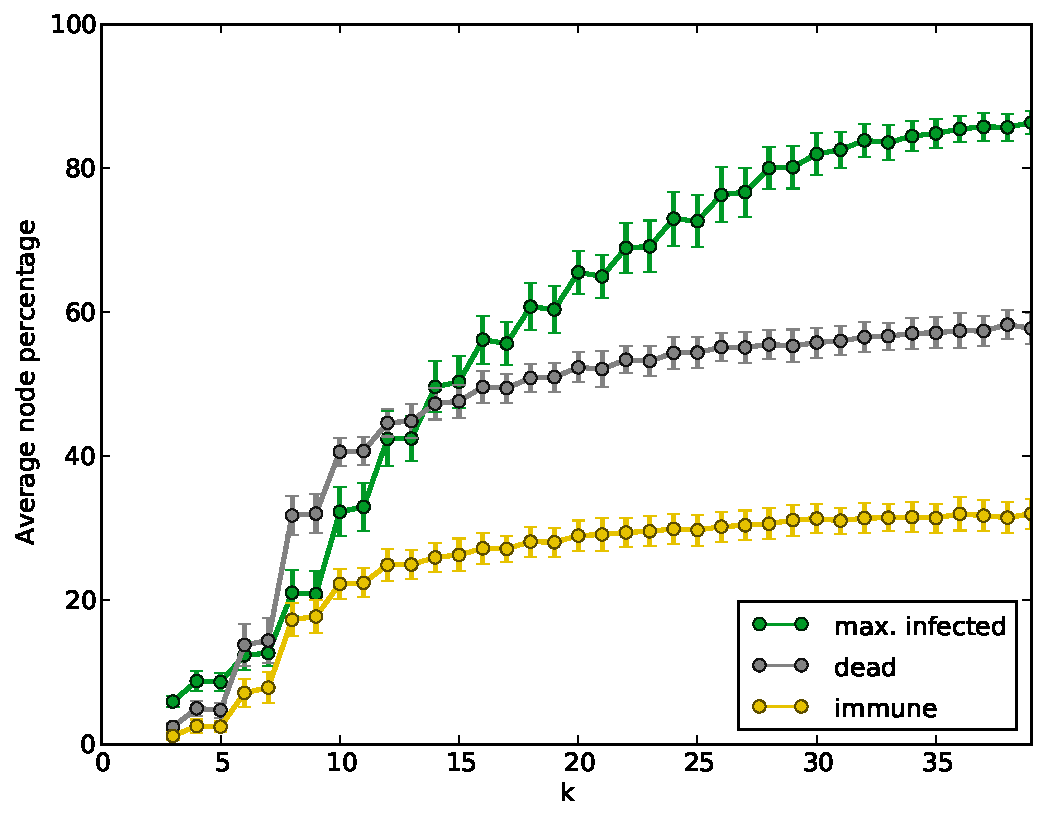
\includegraphics[width=\textwidth]{figures/sum_WS_500_k_01}
  \end{subfigure}
  \caption{Summary plots for WS(500, 25, p) graphs (left) and
    WS(500, k, 0.1) graphs (right) for (100 simulations).}
  \label{fig:ws_sum}
\end{figure}

\begin{figure}[tb]
  \begin{subfigure}[b]{0.5\textwidth}
    \centering
    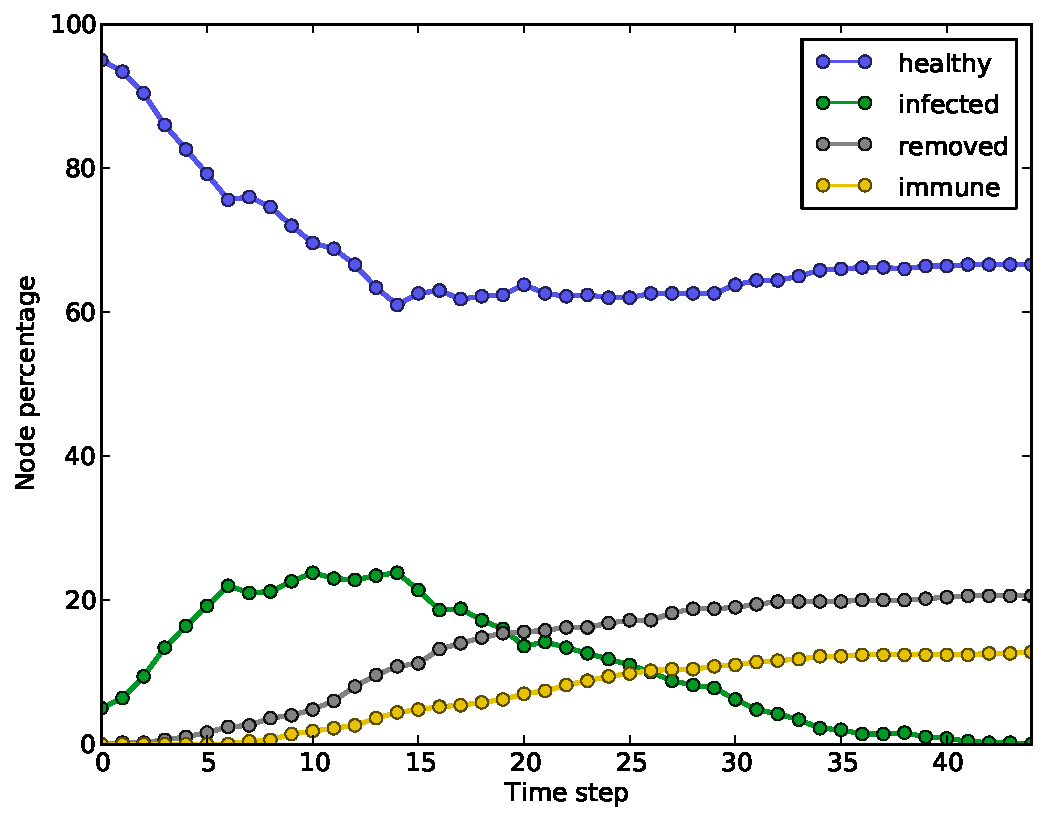
\includegraphics[width=\textwidth]{figures/evo_BA_500_3}
  \end{subfigure}
  \begin{subfigure}[b]{0.5\textwidth}
    \centering
    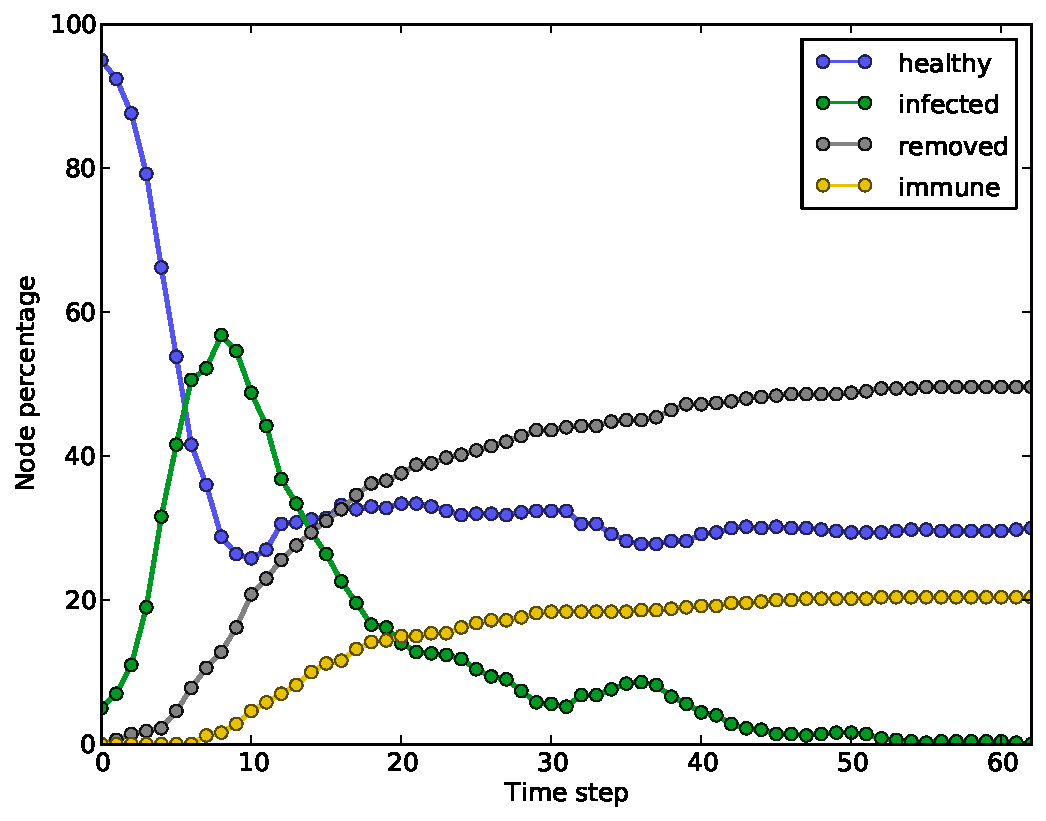
\includegraphics[width=\textwidth]{figures/evo_BA_500_7}
  \end{subfigure}
  \caption{Evolution plots for a BA(500, 3) graph (left) and a
    BA(500, 7) graph (right).}
  \label{fig:ba_evo}
\end{figure}

Two summary plots for the two parameters of the WS model are shown in
\figref{fig:ws_sum}. Concerning the left plot, the fact that the
results seem to be completely independent of the $p$ parameter might
seem surprising at first.
However, increasing the rewiring probability $p$ decreases both the
clustering coefficient and the average path length. If clustering
had no effect, we would expect that the disease spread would increase
with increasing $p$. The fact that it stays constant is a further validation
of the claim that clustering trades-off average shortest path length
when it comes to disease spread. The summary plot with respect to $k$
is easily explained, since increasing the number of initial neighbors
in the WS model, both increases clustering and decreases average
path length.

\begin{wrapfigure}[15]{r}{0.5\textwidth}
  \centering
  \vspace{-15pt}
  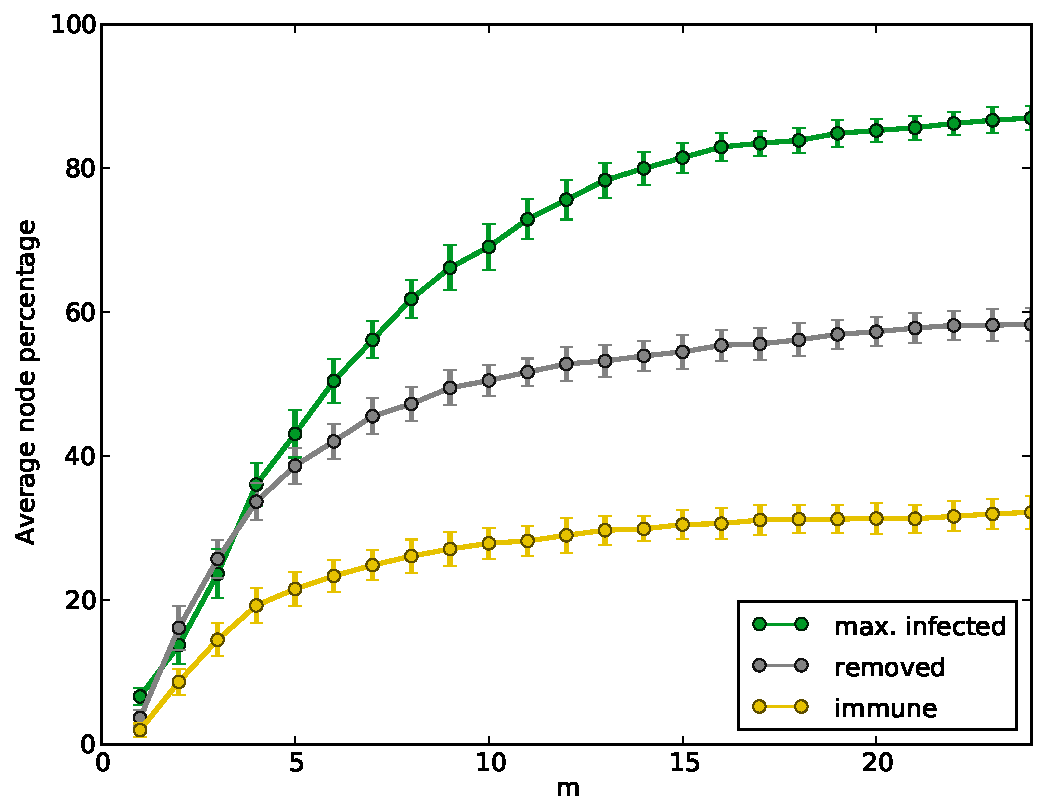
\includegraphics[width=0.5\textwidth]{figures/sum_BA_500_m}
  \vspace{-17pt}
  \caption{Summary plot for BA(500, m).}
  \label{fig:ba_sum}
\end{wrapfigure}

Continuing in the same spirit, I use two sets of BA graph parameters resulting
in the same average
path lengths as the two previous models. From \tabref{tab:metrics}
we can see that the average clustering coefficient for these graphs
are larger than those of the ER graphs, but quite smaller than those
of the BA graphs. The evolution plots of \figref{fig:ba_evo}
are comparable to the ones of the ER graphs in \figref{fig:er_evo},
which means that the preferential attachment process does not seem
to make a difference at this point. Also, the increasing spread with
increasing parameter $m$, shown if the summary plot of
\figref{fig:ba_sum}, is expected.

As mentioned when discussing the BA model, its most important feature
is the creation of ``hubs'', i.e. nodes with a large degree, due to
preferential attachment. To examine the effect of this property
on disease spread, I conducted an additional experiment. I started
with three networks, one of each type, and tuned their parameters
so that their disease spread behavior is similar. Then, I immunized
a number of nodes with the highest closeness
centrality\footnote{Closeness centrality seems to be the most appropriate
centrality measure in this case, since we are talking about a disease which
is spread from a node to its neighbors.}
scores from
each network at the start of each simulation and simulated
the modified networks. The results are shown in the summary plots of
\figref{fig:hub_sum}. Note that, after the immunization of 30 nodes,
in both the ER and the WS models, the average max. infected percentage
has dropped from 80\% to about 70\%, whereas in the BA model the
drop is clearly larger, namely from 80\% to about 60\%. This illustrates
that in the BA model the presence of ``hub'' nodes is more accentuated
than in the other two models.

\begin{figure}[tb]
  \begin{subfigure}[b]{0.5\textwidth}
    \centering
    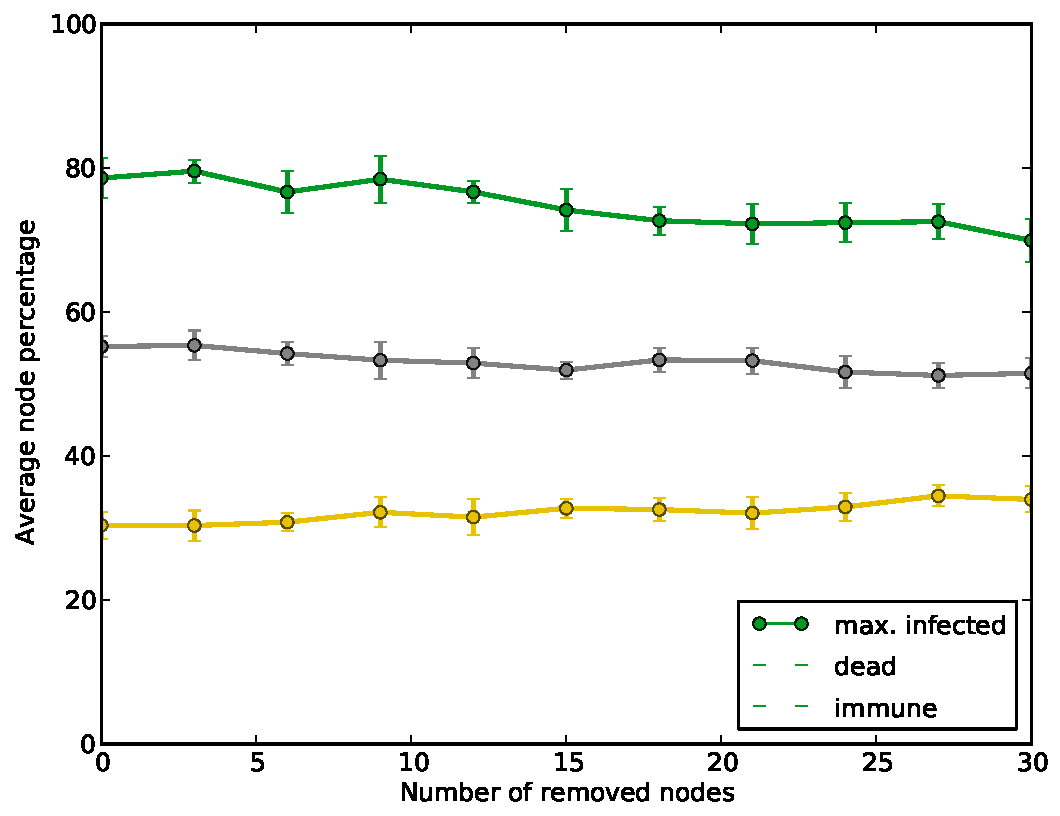
\includegraphics[width=\textwidth]{figures/hubs_ER_500_005}
    \caption{ER(500, 0.05) graph}
  \end{subfigure}
  \begin{subfigure}[b]{0.5\textwidth}
    \centering
    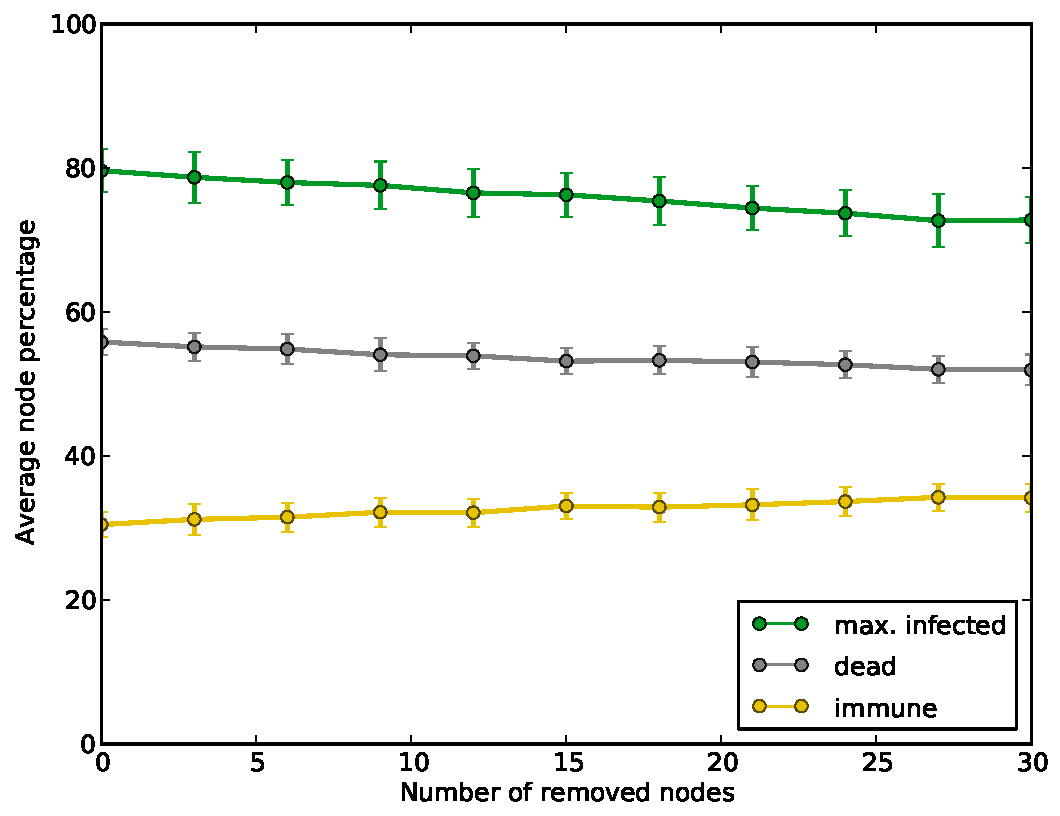
\includegraphics[width=\textwidth]{figures/hubs_WS_500_29_01}
    \caption{WS(500, 29) graph}
  \end{subfigure}
  \begin{subfigure}[b]{0.5\textwidth}
    \centering
    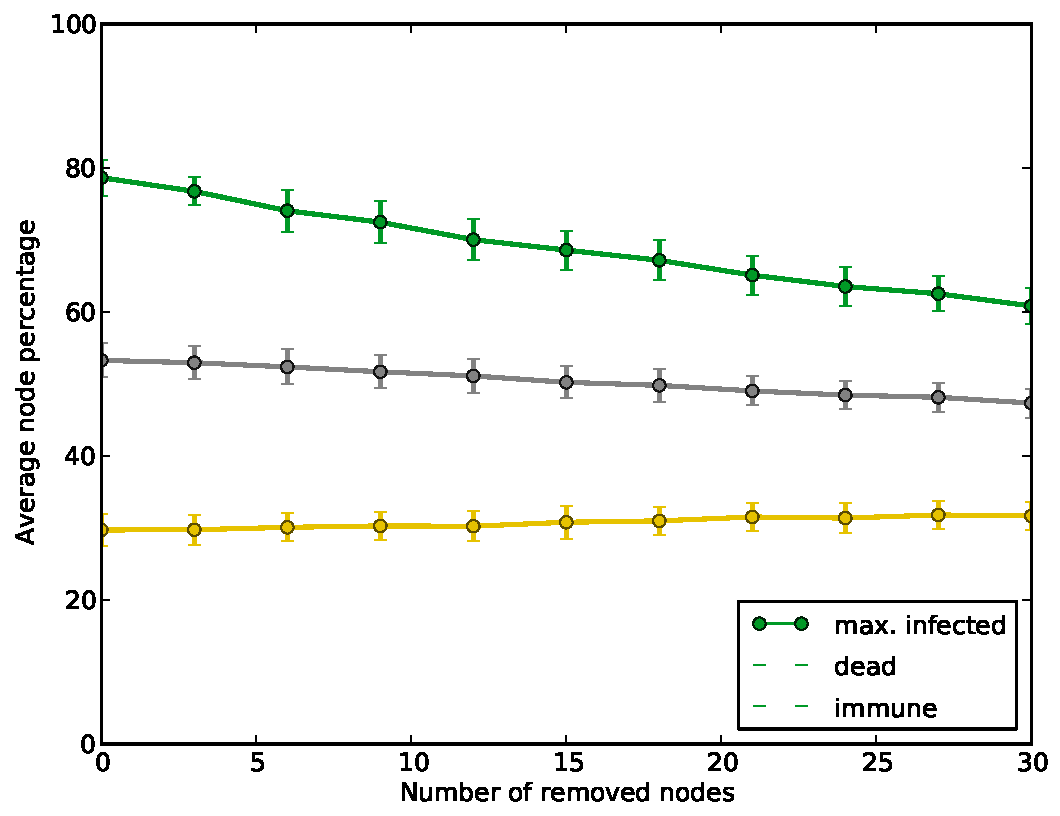
\includegraphics[width=\textwidth]{figures/hubs_BA_500_13}
    \caption{BA(500, 13) graph}
  \end{subfigure}
  \caption{Summary plots when a number of nodes with the highest
    closeness centrality scores are immune.}
  \label{fig:hub_sum}
\end{figure}

\section{Conclusion}
I have presented SIMR, a slightly more complex model than the classic SIR/SIS
ones for modeling disease spread in networks.
I simulated this model on three types of randomly generated graphs using a
Python implementation of it and
noted how the graph types and parameters affect disease spread. Besides the
general (and obvious) observation that larger graph density (equiv. smaller average
shortest path length) increases disease spread, the main observations
are that (1) for ER graphs the point at which disease spread starts to grow
significantly seems to be close to the percolation threshold, (2) graph
clustering tends to boost disease spread, making WS graphs
in general more susceptible to diseases than ER graphs, and (3) containing
disease spread by immunizing targeted nodes is more effective in the BA
model where there are clearer ``hub'' nodes compared to the other models.

The treatment of the subject here was fairly short. It would be interesting
to see how the model parameters affect disease spread and if there are critical
thresholds for their values that make a big difference. Another issue for
investigation would be the effect of dynamic conditions, including randomly
occuring infected nodes and varying network size and structure. Even further,
the dynamics could include game-theoretical concepts, e.g. introduce agents
that try to prevent disease spread (e.g. to model government action).
Finally, the biggest challenge would be to simulate the model on networks
of more realistic size and structure, for example, graph models of a whole city
or country.

\bibliographystyle{plain}
\bibliography{report}

\end{document}
